\documentclass[12pt, a4paper]{report}
\usepackage{style}


\title{Numerical Analysis \\ \textit{Theory}}
\author{Christian Rossi}
\date{Academic Year 2023-2024}

\begin{document}

\maketitle

\newpage

\begin{abstract}
The topics of the course are:
\begin{itemize}
    \item Floating-point arithmetic: different sources of the computational error; absolute vs relative errors; the floating point representation 
        of real numbers; the round-off unit; the machine epsilon; floating-point operations; over- and under-flow; numerical cancellation.
    \item Numerical approximation of nonlinear equations: the bisection and the Newton methods; the fixed-point iteration; convergence analysis 
        (global and local results); order of convergence; stopping criteria and corresponding reliability; generalization to the system of 
        nonlinear equations (hints).
    \item Numerical approximation of systems of linear equations: direct methods (Gaussian elimination method; LU and Cholesky factorizations; 
        pivoting; sparse systems: Thomas algorithm for tridiagonal systems); iterative methods (the stationary and the dynamic Richardson scheme; 
        Jacobi, Gauss-Seidel, gradient, conjugate gradient methods (hints); choice of the preconditioner; stopping criteria and corresponding 
        reliability); accuracy and stability of the approximation; the condition number of a matrix; over- and under-determined systems: the 
        singular value decomposition (hints).
    \item Numerical approximation of functions and data: Polynomial interpolation (Lagrange form); piecewise interpolation; cubic interpolating 
        splines; least-squares approximation of clouds of data.
    \item Numerical approximation of derivatives: finite difference schemes of the first and second order; the undetermined coefficient method.
    \item Numerical approximation of definite integrals: simple and composite formulas; midpoint, trapezoidal, Cavalieri-Simpson quadrature rules; 
        Gaussian formulas; degree of exactness and order of accuracy of a quadrature rule. 
    \item Numerical approximation of ODEs: the Cauchy problem; one-step methods (forward and backward Euler and Crank-Nicolson schemes); 
        consistency, stability, and convergence (hints).
\end{itemize}
\end{abstract}

\newpage

\tableofcontents

\newpage

\chapter{Introduction}
    \section{Numerical analysis and errors}
    Numerical analysis is the field of mathematics dealing with methods to find the solutions of certain mathematical problems with an electronic 
    calculator. It is the intersection between math and computer science. 

    On the other hand, scientific computing also deals with the model formalization and so it needs also engineering knowledge. 
    \begin{figure}[H]
        \centering
        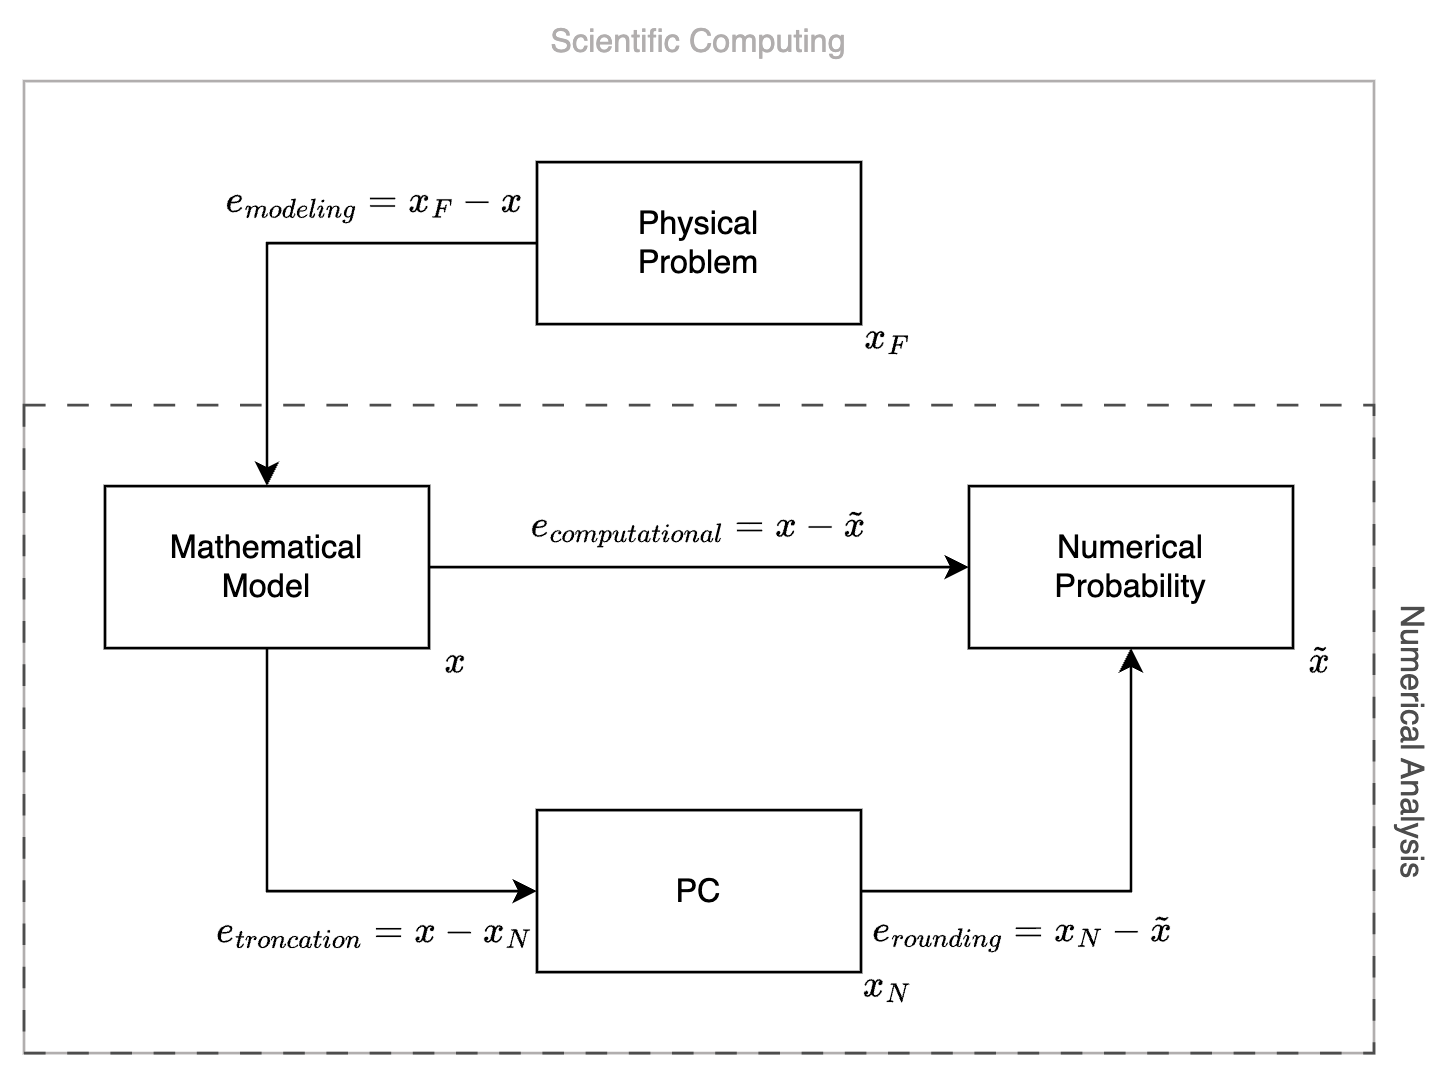
\includegraphics[width=0.75\linewidth]{images/difference.png}
        \caption{Difference between numerical analysis and scientific computing}
    \end{figure}
    As it is possible to see from the diagram every step of the computation have to deal with errors. The possible types of errors are: 
    \begin{itemize}
        \item Absolute: $\left\lvert x - \tilde{x} \right\rvert$
        \item Relative: $\dfrac{\left\lvert x - \tilde{x} \right\rvert}{\left\lvert x \right\rvert}$, where $x \neq 0$
    \end{itemize}
    The relative error is more precise because it compares the error with the measure quantity. 
    \begin{example}
        Let us consider $x=100$ and $\tilde{x}=100.1$. The errors in this case are: 
        \[e_{abs}=\left\lvert x - \tilde{x} \right\rvert=\left\lvert 100 - 100.1 \right\rvert=0.1\]
        \[e_{rel}=\dfrac{\left\lvert x - \tilde{x} \right\rvert}{\left\lvert x \right\rvert}=\dfrac{\left\lvert 100 - 100.1 \right\rvert}{\left\lvert 100 \right\rvert}=0.001\]
        Let us consider $x=0.2$ and $\tilde{x}=0.1$. The errors in this case are: 
        \[e_{abs}=\left\lvert x - \tilde{x} \right\rvert=\left\lvert 0.2 - 0.1 \right\rvert=0.1\]
        \[e_{rel}=\dfrac{\left\lvert x - \tilde{x} \right\rvert}{\left\lvert x \right\rvert}=\dfrac{\left\lvert 0.2 - 0.1 \right\rvert}{\left\lvert 0.2 \right\rvert}=0.5\]
        The result are that the measures have the same absolute error ($10\%$), but the relative error is much grater in the second example ($50\%$ vs $0.1\%$).
        This result proves that the relative error is the most precise.
    \end{example}

    \section{Floating point}
    A calculator can only handle a finite quantity of numbers and compute a finite number of operations. For those reason the set of the real numbers 
    $\mathbb{R}$ is indeed represented by a finite set of machine numbers $\mathbb{F}=\{-\tilde{a}_{min}, \dots , \tilde{a}_{max} \}$ called
    floating points numbers. The function used to find the corresponding value in $\mathbb{F}$ to a number in $\mathbb{R}$ is $fl(x)$ that does an 
    operation called truncation and rounding.

    The set $\mathbb{F}=\mathbb{F}(\beta,t,L,U)$ is characterized by four parameters $\beta,t,L$ and $U$ such that every real number $fl(x) \in \mathbb{F}$ 
    can be written as:
    \[fl(x)=(-1)^s(0.a_1a_2\dots a_t)\beta^e\]
    where:
    \begin{itemize}
        \item $\beta \geq 2$ is the basics, an integer that determines the numeric system. 
        \item $m=(0.a_1a_2\dots a_t)$ is the mantissa.
        \item $e \in \mathbb{Z}$ is the exponent such that $L<e<U$, with $L<0$ and $U>0$. 
        \item $s=\{0,1\}$ is the sign. 
    \end{itemize}
    In the definition of the numbers in the mantissa set we have to set the constraint $a_1 \neq 0$ to ensure the uniqueness of the representation. In this case we say that the number
    is normalized. 

    The set of floating points has the following characteristic values are:
    \begin{itemize}
        \item Machine epsilon, that is the distance between one and the smallest floating point number greater than one, and it is equal to: 
            \[\epsilon_M=\beta^{1-t}\]
        \item Round-off error, that is the relative error that is committed when substituting $x \in \mathbb{R}-\{0\}$ with his corresponding 
            $fl(x) \in \mathbb{F}$. It is limited by: 
            \[\dfrac{\left\lvert x-fl(x) \right\rvert}{\left\lvert x \right\rvert }\leq \dfrac{1}{2}\epsilon_M\]
            where $x \neq 0$.
        \item The biggest and the smallest numbers in the set are found with the formula:
            \[x_{min}=\beta^{L-1}\]
            \[x_{max}=\beta^U(1-\beta^{-t})\]
    \end{itemize}
    \begin{example}
        In MATLAB the floating point set is defined with the following variables:
        \[(\beta=2,t=53,L=-1021,U=1024)\] 
        With the command $eps$ we can find the machine epsilon, that in MATLAB case is:
        \[\epsilon_M=2.22 \cdot 10^{-16}\]
        With the command $realmin$ and $realmax$ we can find the smallest and the largest numbers representable that are equal to:
        \[x_{min}=2.225073858507201 \cdot 10^{-308}\]
        \[x_{max}=1.797693134862316 \cdot 10^{308}\]
    \end{example}
    Since not all the numbers in the $\mathbb{R}$ set are also in the $\mathbb{F}$ set, in the second one there is no continuity. It is possible to 
    demonstrate that while we are increasing the values of the numbers we are also increasing the distance between two consecutive numbers in $\mathbb{F}$.
    \begin{example}
        Let us consider the floating number set $\mathbb{F}(2,2,-1,2)$. The characteristic values of this set are: 
        \begin{itemize}
            \item $\epsilon_M=\beta^{1-t}=0.5$.
            \item $x_{min}=\beta^{L-1}=0.25$.
            \item $x_{max}=\beta^U(1-\beta^t)=3$.
            \item $\#\mathbb{F}=2 \beta^{t-1}(\beta -1)(U-L+1)+1=16$. 
        \end{itemize}
        The exponent can have the values $-1,0,1$ and $2$. The mantissa will be like $(a_1a_2)_{\beta}$ because $t=2$. The possible positive values are
        reported in the figure. 
        \begin{figure}[H]
            \centering
            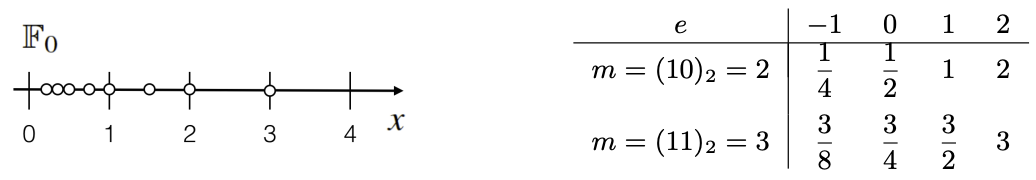
\includegraphics[width=0.9\linewidth]{images/numbers.png}
        \end{figure}
    \end{example}
    The other important aspect is that the passage between the two sets causes the loss of two important properties such as associativity end the 
    neutral number for the sum. 

\newpage 
\chapter{Nonlinear equations}
    \section{Introduction}
    To solve a nonlinear equation $f(x)$ we have to find $\alpha \in \mathbb{R}$ that is a zero of $f$ such that $f(\alpha)=0$.
    \begin{definition}
        The point $\alpha$ is said to be a \emph{zero with multiplicity $m$} if:
        \begin{itemize}
            \item $f(\alpha)=f^{'}(\alpha)=\dots=f^{\left(m-1\right)}(\alpha)=0$.
            \item $f^{\left(m\right)}(\alpha) \neq 0$.
        \end{itemize}
    \end{definition}
    If $m$ is odd the function changes sign across the zero. It does not change the sign if $n$ is even. 

    \section{Iterative methods}
    The set of all the polynomials of degree $n$ is denoted by the symbol $\mathbb{P}_n$ that contains all the polynomial that have a grade less or equal to $n$.
    \begin{theorem}[Abel-Ruffini theorem]
        There is no solution in radicals to general polynomial equations of degree five or higher with arbitrary coefficients. 
    \end{theorem}
    So, to solve polynomials with a degree higher than four we need to use the iterative methods. The general idea of those methods is the following:
    \begin{enumerate}
        \item Select an arbitrary initial value $x^{(0)}$ called initial guess, that is a hypothetical value for $\alpha$.
        \item Use the selected value as an input for a black-box function.
        \item Use the output of the black-box function as the new $x^{(0)}$ and return to point one. 
    \end{enumerate}
    After some iterations (that depends on the chosen method) we will have a set of values $\{ x^{(n)} \}$ convergent such that:
    \[ \lim_{n \rightarrow \infty} = \alpha\]
    and the error related to the value found for $\alpha$ is equal to: 
    \[ \lim_{n \rightarrow \infty}e^n = 0\]
    That Rightarrow that the error can be also written as: 
    \[e^n=\alpha-x^{(n)}\]
    All the methods we are going to see constructs a sequence $x^{(1)},x^{(2)},\dots,x^{(n)}$ of numbers that hopefully converges to $\alpha$:
    \[ \lim_{k \rightarrow + \infty} \left\lvert x^{(k)}-\alpha \right\rvert =0\]
    \begin{definition}[order of convergence]
        An iterative method for the approximation of the zero $\alpha$ of the function $f(x)$ is convergent with order $q$ if and only if for $k > k_0$:
        \[\left\lvert x^{(k)} - \alpha \right\rvert \leq c {\left\lvert x^{(k+1)} - \alpha \right\rvert}^q  \]
        We can have two cases:
        \begin{itemize}
            \item If $q=1$ it is called linear convergence and there are the constraint $0<c<1$.
            \item If $q>1$, $c$ can be any positive number grater than zero. 
        \end{itemize}
    \end{definition}

    \section{Stopping conditions}
    The iterative methods need a stopping criterion. It can be on four possible conditions: 
    \begin{itemize}
        \item On the error, stops if $\left\lvert x^{(k)}-\alpha \right\rvert \leq \epsilon_e$.
        \item On the residual, stops if $\left\lvert f\left(x^{(k)}\right) \right\rvert \leq \epsilon_r$. 
        \item On the step length, stops if $\left\lvert x^{(k)}-x^{(k-1)} \right\rvert \leq \epsilon_s$. 
        \item On the max numbers of iterations, stops if $k \leq k_{max}$. 
    \end{itemize}
    If none of the first three stopping criterions are satisfied, it means that there are no convergence. 

    \section{Bisection method}
    \begin{theorem}[zeros of continuous functions]
        Let $f(x)$ be a continuous function on the interval $I=(a,b)$, that is $f \in C^0([a,b])$. 
        If $f(a)f(b)<0$, then there exists at least one zero $\alpha \in I$ of $f(x)$. 
    \end{theorem}
    Let us assume that exist a unique zero, and let us call it $\alpha$. 
    The strategy of the bisection method is to have the given interval and select a sub-interval where $f$ features a sign change. Following 
    such procedure it is guaranteed that every interval selected this way will contain $\alpha$. The sequence $\{x^{(k)}\}$ of the midpoints of 
    these sub-intervals will inevitably tend to $\alpha$ since the length of the sub-intervals tends to zero as $k$ tends to infinity.
    We have that:
    \[\left\lvert x^{(k)} - \alpha \right\rvert \leq \dfrac{1}{2} \left\lvert b^{(k)}-a^{(k)} \right\rvert \]
    So, since the first part of the equation is similar to the condition on the error, we have that the stopping criterion will be: 
    \[\left\lvert b^{(k)}-a^{(k)} \right\rvert \leq 2 \epsilon_e\]
    Now that we have the tolerance $\epsilon$ we can find that:
    \[k_{min}= \left\lceil {\log_2{\left( \dfrac{\left\lvert b-a \right\rvert}{\epsilon} \right)} - 1}\right\rceil \]
    The inputs for the algorithm are: a function $f \in C(\mathbb{R})$ and an interval $[a,b]$ such that $f(a)f(b) \leq 0$. 
    \begin{algorithm}[H]
        \caption{Algorithm for the bisection method}
            \begin{algorithmic}[1]
                \For {$k=0,1,\dots,n$}
                    \State $x^{(k)}=\dfrac{a+b}{2}$
                    \If {$\left\lvert b^{(k)}-a^{(k)} \right\rvert \leq 2 \epsilon_e$}
                        \State \Return $x^{(k)}$
                    \ElsIf {$f(x^{(k)})f(a) < 0$}
                        \State $b \leftarrow x^{(k)}$
                    \Else 
                        \State $a \leftarrow x^{(k)}$
                    \EndIf
                \EndFor
            \end{algorithmic}
    \end{algorithm}
    The pros are: 
    \begin{itemize}
        \item I can control the maximal error.
        \item Convergence is guaranteed.
        \item Use only evaluation of $f$
    \end{itemize}
    The cons are: 
    \begin{itemize}
        \item Work only if $f$ changes sign. 
        \item Convergence is slow.
    \end{itemize}
   
    \section{Newton method}
    The sign of the given function $f$ at the endpoints of the sub-intervals is the only information exploited by the bisection method. A more efficient method can be constructed 
    by exploiting the values attained by $f$ and its derivative. If $f$ is differentiable we have that: 
    \[y(x)=f(x^{(k)})+f^{'}(x^{(k)})(x-x^{(k)})\]
    provides the equation of the tangent to the curve $(x,f(x))$ at the point $x^{(k)}$. If we pretend that $x^{(k+1)}$ is such that $f(x^{(k+1)})=0$, we obtain:
    \[x^{(k+1)}=x^{(k)}-\dfrac{f(x^{(k)})}{f^{'}(x^{(k)})} \:\:\:\:\:\: k \geq 0\]
    provided $f^{'}(x^{(k)}) \neq 0$. This method is known as Newton's method and corresponds to computing the zero of $f$ locally replacing $f$ by its tangent line. 

    Obviously, this method converges in a single step when $f$ is linear. 

    The Newton method in general doe not converge for all possible choices of $x^{(0)}$, but only for those values of $x^{(0)}$ which are sufficiently close to $\alpha$. Since we 
    don't know the value of $\alpha$ a possible initial value $x^{(0)}$ can be obtained by resorting to a few iterations of the bisection method or through an investigation of the 
    graph of $f$. 

    If $f \in C^2(\mathbb{R})$, $f^{'}(\alpha) \neq 0$, and $x^{(0)}$ is taken sufficiently near $\alpha$ the Newton method converges quadratically. In the case of zeros with 
    multiplicity $m$ larger than one Newton method converges linearly. To avoid this degradation it is possible to use the modified Newton method:
    \[x^{(k+1)}=x^{(k)}-m\dfrac{f(x^{(k)})}{f^{'}(x^{(k)})} \:\:\:\:\:\: k \geq 0\]
    provided $f^{'}(x^{(k)}) \neq 0$.

    Another modification to this method is the quasi-Newton method that uses a derivative by finite difference: 
    \[f^{'}(x^{(k)}) \simeq \dfrac{f(x^{(k)}+h)-f(x^{(k)})}{h}\]

    The inputs for the algorithm are: a function $f \in C^1(\mathbb{R})$ and an initial guess $x^{(0)} \in \mathbb{R}$. 
    \begin{algorithm}[H]
        \caption{Algorithm for the basic Newton method}
            \begin{algorithmic}[1]
                \For {$k=0,1,\dots,n$}
                    \State $x^{(k+1)}=x^{(k)}-\dfrac{f(x^{(k)})}{f^{'}(x^{(k)})}$
                    \If {$k>k_{max} \lor \left\lvert x^{(k)}-x^{(k-1)} \right\rvert \leq \epsilon_s \lor \left\lvert f\left(x^{(k+1)}\right) \right\rvert \leq \epsilon_r$}
                        \State \Return $x^{(k+1)}$
                    \EndIf
                \EndFor
            \end{algorithmic}
    \end{algorithm}
    The pros are: 
    \begin{itemize}
        \item Fast convergence. 
        \item Works also for zeros with even multiplicity. 
    \end{itemize}
    The cons are: 
    \begin{itemize}
        \item Require computation of the derivative. 
        \item Choice of the right $x^{(0)}$. 
    \end{itemize}

    \section{Secant method}
    For the computation of the zeros of a function $f$ whose derivative is not available in analytical form, the Newton method cannot be applied. However, we should be able to 
    compute the function $f$ at any arbitrary point, and we could replace the exact value $f^{'}(x^{(k)})$ with an incremental ratio based on previously computed values of $f$. The 
    secant method exploits this strategy and converges super-linearly ($q=1.6$). 

    The inputs for the algorithm are: two initial guesses $x^{(0)} \in \mathbb{R}$ and $x^{(1)} \in \mathbb{R}$. 
    \begin{algorithm}[H]
        \caption{Algorithm for the secant method}
            \begin{algorithmic}[1]
                \For {$k=0,1,\dots,n$}
                    \State $x^{(k+1)}=x^{(k)}-f(x^{(k)})\dfrac{x^{(k)}-x^{(k-1)}}{f(x^{(k)})-f(x^{(k-1)})}$
                    \If {$k>k_{max} \lor \left\lvert x^{(k)}-x^{(k-1)} \right\rvert \leq \epsilon_s \lor \left\lvert f\left(x^{(k+1)}\right) \right\rvert \leq \epsilon_r$}
                        \State \Return $x^{(k+1)}$
                    \EndIf
                \EndFor
            \end{algorithmic}
    \end{algorithm}

    \section{Fixed point method}
    Given a function $\phi:[a,b] \rightarrow \mathbb{R}$, find $\alpha \in [a,b]$ such that $\alpha=\phi(\alpha)$. If such an $\alpha$ exists it will be called a fixed point of 
    $\phi$, and it could be computed by the following algorithm: 
    \[x^{(k+1)}=\phi(x^{(k)}) \:\:\:\:\:\: k \geq 0\]
    where $x^{(0)}$ is an initial guess. This algorithm is called fixed point iteration and $\phi$ is said to be the iteration function. 
    \begin{theorem}[Lipschitz continuity]
        \begin{enumerate}
            \item Let us suppose that $\phi(x)$ is continuous in $[a,b]$ and such that $\phi(x) \in [a,b]$ for every $x \in [a,b]$; then, there exists at least a fixed point 
                $\alpha \in [a,b]$.
            \item Moreover, if 
                \[\exists L < 1 \textnormal{such that} \left\lvert \phi(x_1)-\phi(x_2) \right\rvert \leq L\left\lvert x_1-x_2 \right\rvert  \:\:\:\:\:\: \forall x_1,x_2 \in [a,b]\]
                then there exists a unique fixed point $\alpha \in [a,b]$ of $\phi$ and the sequence converges to $\alpha$, for any choice of initial guess $x^{(0)} \in [a,b]$.
        \end{enumerate}
    \end{theorem}
    \begin{proof}[of the first proposition]
        The function $g(x)= \phi(x)-x$ is continuous in $[a,b]$ and, thanks to assumption made on the range of $\phi$, it holds $g(a) = \phi(a)-a \geq 0$ and $g(b) = \phi(b)-b \geq 0$.
        By applying the theorem of zeros of continuous functions, we can conclude that $g$ has at least one zero in $[a,b]$. 
    \end{proof}
    \begin{proof}[of the second proposition]
        Indeed, should two different fixed points $\alpha_1$ and $\alpha_2$ exist, then: 
        \[\left\lvert \alpha_1-\alpha_2 \right\rvert = \left\lvert \phi(\alpha_1)-\phi(\alpha_2) \right\rvert \leq L \left\lvert \alpha_1-\alpha_2 \right\rvert < 
        \left\lvert \alpha_1-\alpha_2 \right\rvert\]
        which cannot be. We prove now that the sequence $x^{(k)}$ converges to the unique fixed point $\alpha$ when $k \rightarrow \infty$, for any choice of initial guess $x^{(0)} 
        \in [a,b]$. It holds: 
        \[\dfrac{\left\lvert x^{(k)}-\alpha \right\rvert}{\left\lvert x^{(0)}-\alpha \right\rvert} \leq L^k\]
        Passing to the limit as $k \rightarrow \infty$, we obtain $\lim_{k \rightarrow \infty}{\left\lvert x^{(k)}-\alpha \right\rvert}=0$, which is the desired result. 
    \end{proof}
    In practice it is often very difficult to choose a priori an interval $[a,b]$ for which the assumptions of previous proposition are fulfilled. In such cases the following local
    convergence result will be useful. 
    \begin{theorem}[Ostrowski]
        Let $\alpha$ be a fixed point of a function $\phi$ which is continuous and continuously differentiable in a suitable neighborhood $\mathcal{J}$ of $\alpha$. If 
        $\left\lvert \phi^{'}(\alpha) \right\rvert < 1$, then there exists $\delta > 0$ for which $\{x^{(k)}\}$ converges to $\alpha$, for every $x^{(0)}$ such that 
        $\left\lvert x^{(0)}-\alpha \right\rvert < \delta$. Moreover, it holds: 
        \[\lim_{k \rightarrow \infty}\dfrac{x^{(k+1)}-\alpha}{x^{(k)}-\alpha}=\phi^{'}(\alpha)\]
    \end{theorem}

    For the hypothesis of the Ostrowski theorem we have that: 
    \[\exists \delta | \left\lvert \phi^{'}(\alpha) \right\rvert < 1 \:\:\:\:\:\: \forall x \left\lvert x - \alpha \right\rvert < \delta\]
    We will call this interval $I_{\delta}$. If I choose a point $x$ inside this interval, I will have that $\phi(x) \in I_{\delta}$. 
    \begin{proof}
        Let us take $\left\lvert \phi(x)-\alpha \right\rvert$, where it is satisfied the relation $\left\lvert x- \alpha \right\rvert < \delta$. We have
        \[\left\lvert \phi(x)-\alpha \right\rvert=\left\lvert \phi(x)-\phi(\alpha) \right\rvert \leq \left\lvert \phi^{'}(\xi)(x-\alpha) \right\rvert \]
        So, we have that $\xi$ is between $x$ and $alpha$, and so it holds $\xi \in I_{\delta}$. At the meantime we have by hypothesis that: 
        \[\left\lvert \phi^{'}(\xi) \right\rvert < 1\]
        Now we can write 
        \[\left\lvert \phi^{'}(\xi)(x-\alpha) \right\rvert = \left\lvert \phi^{'}(\xi) \right\rvert \left\lvert x-\alpha \right\rvert \leq \left\lvert x-\alpha \right\rvert < \delta\]
        In the end we found that: 
        \[\left\lvert \phi(x)-\alpha \right\rvert < \delta\]
        So we have proved that $\phi(x) \in I_{\delta}$. 
    \end{proof}
    \begin{proof}[Ostrowski]
        Thanks to the Lagrange theorem, for any $k \geq 0$, there exists a point $\xi_k$ between $x^{(k)}$ and $\alpha$ such that $\left\lvert x^{(x)}-\alpha\right\rvert =
        \left\lvert \phi(x^{(x)})-\phi(\alpha)\right\rvert = \left\lvert \phi^{'}(\xi_k)(x^{(x)}-\alpha)\right\rvert $. We found that $\xi_k$ is between $x^{(k)}$ and $x^{(k+1)}$. 
        So if $x^{(k)} \in I_{\delta}$, for the previous proof I have that also $x^{(k+1)} \in I_{\delta}$ and $\xi_k \in I_{\delta}$. And so we have that: 
        \[\dfrac{\left\lvert x^{(k+1)}-\alpha\right\rvert }{\left\lvert x^{(k)}-\alpha\right\rvert }=\left\lvert \phi^{'}(\xi_k)\right\rvert \]
        But since $\xi_k \rightarrow \alpha$, we have the convergence formula. 
    \end{proof}
    The fixed point iteration converge at least linearly. When $\left\lvert \phi^{'}(\alpha) \right\rvert > 1$, if $x^{(k)}$ is sufficiently close to $\alpha$, such that 
    $\left\lvert \phi^{'}(x^{(k)}) \right\rvert > 1$, then $\left\lvert \alpha - x^{(k+1)} \right\rvert > \left\lvert \alpha - x^{(k)} \right\rvert$, and the sequence cannot 
    converge to the fixed point. On the contrary, when $\left\lvert \phi^{'}(\alpha) \right\rvert = 1$, non conclusion can be drawn since either convergence or divergence could 
    take place, depending on the properties of the iteration function $\phi^{'}(x)$. 
    \begin{proposition}
        Assume that all hypothesis of Ostrowski's theorem are satisfied. In addition, assume that $\phi$ is twice continuously differentiable and that $\phi^{'}(\alpha)=0$ and 
        $\phi^{''}(\alpha) \neq 0$. Then, the fixed point iteration converge with order two and:
        \[\lim_{k \rightarrow \infty}\dfrac{x^{(k+1)}-\alpha}{\left(x^{(k)}-\alpha\right)^2}=\dfrac{1}{2}\phi^{''}(\alpha)\]
    \end{proposition}
    Given a simple zero such that $f(\alpha)=0$ we can use the fixed point method to derive the Newton method: 
    \[\phi_N(x)=x-\dfrac{f(x)}{f^{'}(x)}\]
    If we derive the previous function we obtain:
    \[\phi^{'}_N(x)=\dfrac{f(x)f^{''}(x)}{\left[f^{'}(x)\right]^2}\]
    And we can say that: 
    \[\phi^{'}_N(\alpha)=\dfrac{f(\alpha)f^{''}(\alpha)}{\left[f^{'}(\alpha)\right]^2}=0\]
    \begin{proof}
        We can note that the denominator is not null (the zero is simple, so the first derivative is not null). We assumed that $f(\alpha)=0$, and we can say nothing about 
        $f^{''}(\alpha)$. But since we have 
        \[\phi^{'}_N(\alpha)=\dfrac{f(\alpha)f^{''}(\alpha)}{\left[f^{'}(\alpha)\right]^2}=\dfrac{0 \cdot n}{n}=\dfrac{0}{n}=0\]
        We have that the function evaluated in $\alpha$ is zero. 
    \end{proof}

    The stopping criterion for the fixed point iteration method is: 
    \[\left\lvert x^{(k+1)}-x^{(k)} \right\rvert \leq \epsilon_s\]
    \begin{proof}[not null derivative]
        We have that the error in a certain iteration is: 
        \[\left\lvert x^{(k+1)} - \alpha \right\rvert = \left\lvert \phi(x^{(k)}) - \phi(\alpha) \right\rvert \leq \left\lvert \phi^{'}(\xi_k)\right\rvert \left\lvert x^{(k)} - \alpha\right\rvert \]
        Then I add and subtract $x^{(k+1)}$: 
        \[\left\lvert \phi^{'}(\xi_k)\right\rvert \left\lvert x^{(k)} - \alpha + x^{(k+1)} - x^{(k+1)}\right\rvert\]
        Applying the triangular inequality we obtain: 
        \[\left\lvert \phi^{'}(\xi_k)\right\rvert 
        \left\lvert x^{(k)} - \alpha + x^{(k+1)} - x^{(k+1)}\right\rvert \leq 
        \left\lvert \phi^{'}(\xi_k)\right\rvert 
        \left\lvert x^{(k+1)} - \alpha \right\rvert 
        \left\lvert x^{(k)} - x^{(k+1)} \right\rvert\]
        From where we can derive: 
        \[\left( 1-\left\lvert \phi^{'}(\xi_k)\right\rvert \right) \left\lvert x^{k+1}-\alpha \right\rvert \leq \left\lvert \phi^{'}(\xi_k)\right\rvert \left\lvert x^{(k+1)} - x^{(k)} \right\rvert\]
        That is: 
        \[ \left\lvert x^{(k+1)} - \alpha \right\rvert \leq \dfrac{\phi^{'}(\xi_k)}{1-\left\lvert \phi^{'}(\xi_k)\right\rvert} \left\lvert x^{(k+1)} - x^{(k)} \right\rvert\]
    \end{proof}
    \begin{proof}[null derivative]
        We have that: 
        \[\left\lvert x^{(k+1)} - \alpha \right\rvert \leq \left\lvert x^{(k+1)} - \alpha + x^{(k)} - x^{(k)}\right\rvert \leq \left\lvert x^{(k+1)}-x^{(k)}\right\rvert \left\lvert \phi{x^{(k+1)}}-\phi(\alpha)\right\rvert\]
        That is less or equal than:
        \[ \left\lvert x^{(k+1)} - x^{(k)} \right\rvert 
        + 
        \left\lvert \phi^{'}(\xi_k) \right\rvert  
        \left\lvert x^{(k+1)} - \alpha \right\rvert\]
        But for hypothesis we have that $\phi^{'}(\alpha)=0$ we obtain: 
        \[ \left\lvert x^{(k+1)} - \alpha \right\rvert \leq \left\lvert x^{(k+1)} - x^{(k)} \right\rvert\]
    \end{proof}

    \section{Aitken method}
    We have that: 
    \[x^{(k+1)}-\alpha=\phi(x^{(k+1)})-\phi(\alpha)=\lambda_k\left( x^{(k+1)}-\alpha \right)\]
    And we know that $\lambda_k$ is the first derivative of $\phi$ in a certain point $\xi$. If I know $\lambda_k$ I have that: 
    \[\alpha=\dfrac{\phi(x^{(k)})-\lambda_k x^{k}}{1-\lambda_k}\]
    We also have that the quantity 
    \[A_k=\dfrac{\phi(\phi(x^{(k)}))-\phi(x^{(k)})}{\phi(x^{(k)})-x^{(k)}}\]
    is a good approximation of $\lambda_k$, so I can replace $\lambda_k$ with $A_k$. By substituting, we obtain the formula used in the Aitken method. 
    \begin{algorithm}[H]
        \caption{Algorithm for the Aitken method}
            \begin{algorithmic}[1]
                \For {$k=0,1,\dots,n$}
                    \State $x^{(k+1)}=x^{(k)}-\dfrac{\left[ \phi(x^{(k)})-x^{(k)} \right]^2}{\phi(\phi(x^{(k)}))-2\phi(x^{(k)})+x^{(k)}}$
                    \If {stopping criterion is satisfied}
                        \State \Return $x^{(k+1)}$
                    \EndIf
                \EndFor
            \end{algorithmic}
    \end{algorithm}
    \begin{theorem}
        Let $\phi(x)=x-f(x)$ and $f(\alpha)$ be a simple zero. Let $\phi^{(k)}$ converge to the first order to $\alpha$, then $\phi_A$ converge to the second order. 

        If $\phi(x)$ converges with order $p$ and $f(x)$ is still a simple zero, then $\phi_A$ converges with order $2p-1$. 
    \end{theorem}
    Sometimes $\phi_A$ converges even if $\phi$ does not. 

    \section{Systems of nonlinear equations}
    \subsection{Newton method}
    Let us consider a system of nonlinear equations of the form
    \[\begin{cases}
        f_1(x_1,x_2,\dots,x_n)=0 \\
        f_2(x_1,x_2,\dots,x_n)=0 \\
        \vdots                   \\
        f_n(x_1,x_2,\dots,x_n)=0 
    \end{cases}\]
    where $f_1,\dots,f_n$ are nonlinear functions. Setting $\boldsymbol{f}=(f_1,\dots,f_n)^T$ and $\boldsymbol{x}=(x_1,\dots,x_n)^T \in \mathbb{R}^d$, the system can be written in a compact way as: 
    \[\boldsymbol{f}(\boldsymbol{x})=\boldsymbol{0}\]
    In order to extend Newton's method to the case of a system, we replace the first derivative of the scalar function $f$ with the Jacobian matrix $J_{\boldsymbol{f}}$ of the vectorial 
    function $\boldsymbol{f}$ whose components are: 
    \[(\boldsymbol{J}_{\boldsymbol{f}})_{ij}=\dfrac{\partial f_1}{\partial x_1} \:\:\:\:\:\: i,j=1,\dots,n\]

    The input of the algorithm is the initial guess $\boldsymbol{x}^{(0)}$. 
    \begin{algorithm}[H]
        \caption{Algorithm for the Newton method for systems}
            \begin{algorithmic}[1]
                \For {$k=0,1,\dots,n$}
                    \State $\textnormal{solve  } \boldsymbol{J}_{\boldsymbol{f}}(\boldsymbol{x}^{(k)})\boldsymbol{\delta}\boldsymbol{x}^{(k)}=-\boldsymbol{F}(\boldsymbol{x}^{(k)})$
                    \State $\boldsymbol{x}^{(k+1)} \leftarrow \boldsymbol{x}^{(k)}+\boldsymbol{\delta}\boldsymbol{x}^{(k)}$
                    \If {$\left\lVert \boldsymbol{\delta}\boldsymbol{x}^{(k+1)} \leq \epsilon \right\rVert \lor \left\lVert \boldsymbol{F}(\boldsymbol{x}^{(k+1)}) \leq \epsilon_r \right\rVert$}
                        \State \Return $x^{(k+1)}$
                    \EndIf
                \EndFor
            \end{algorithmic}
    \end{algorithm}
    The computation of the Jacobian matrix $\boldsymbol{J}_{\boldsymbol{f}}$ can be expensive if the number of equations $d$ is relatively large. To simplify the computation of this matrix
    it is possible to use the approximation with finite difference, that is: 
    \[(\boldsymbol{J}_{\boldsymbol{f}})_{ij} \approx \dfrac{f_i(x_1^{k},\dots,x_{j-1}^{k},x_{j+h}^{k},x_{j+1}^{k},\dots,x_{d}^{k})-f(\boldsymbol{x}_{k})}{h}\]
    But also this method is costly. There are other method used to approximate the Jacobian that are less expensive that are called quasi-Newton methods. The most important 
    quasi-Newton method used for this purpose is called Broyden. 

    \subsection{Broyden method}
    The secant method can be adapted to the solution of systems of nonlinear equations still featuring super-linear rate of convergence. The idea consists in replacing the Jacobian 
    matrix $\boldsymbol{J}_{\boldsymbol{f}}(\boldsymbol{x}^{(k)})$ (for $k \geq 0$) of Newton's method with suitable matrices $B_k$, recursively defined starting from a convenient matrix $B_0$, 
    representing a suitable approximation of $\boldsymbol{J}_{\boldsymbol{f}}(\boldsymbol{x}^{(0)})$.
    
    The starting idea is to replace $\boldsymbol{I}_k$ with a matrix $\boldsymbol{B}_k$ that satisfies the equation: 
    \[\boldsymbol{B}_k\left(\boldsymbol{x}_k-\boldsymbol{x}_{k-1}\right)=\boldsymbol{F}(\boldsymbol{x}_k)-\boldsymbol{F}(\boldsymbol{x}_{k-1})(S)\]
    Since there are infinite matrices that satisfies the previous equation, the idea of Broyden was to choose $\boldsymbol{B}_k$ so that it satisfies $(S)$ and minimizes: 
    \[\min{\left\lVert \boldsymbol{B}_k-\boldsymbol{B}_{k-1} \right\rVert_{\boldsymbol{F}}^{2}}\]

    The input of the algorithm is the initial guess $\boldsymbol{x}^{(0)} \in \mathbb{R}^n$ and a given $\boldsymbol{B}_0 \in \mathbb{R}^{n \times n}$ (we usually set $\boldsymbol{B}_0=\boldsymbol{I}$). 
    \begin{algorithm}[H]
        \caption{Algorithm for the Broyden method for systems}
            \begin{algorithmic}[1]
                \For {$k=0,1,\dots,n$}
                    \State $\textnormal{solve  } \boldsymbol{B}_k\boldsymbol{\delta}\boldsymbol{x}^{(k)}=-\boldsymbol{f}(\boldsymbol{x}^{(k)})$
                    \State $\boldsymbol{x}^{(k+1)} \leftarrow \boldsymbol{x}^{(k)}+\boldsymbol{\delta}\boldsymbol{x}^{(k)}$
                    \State $\boldsymbol{\delta}\boldsymbol{f}^{(k)} \leftarrow \boldsymbol{f}(\boldsymbol{x}^{(k+1)})+\boldsymbol{f}(\boldsymbol{x}^{(k)})$
                    \State $B_{k+1}=B_k+\dfrac{\left(\boldsymbol{\delta}\boldsymbol{f}^{(k)}-B_k\boldsymbol{\delta}\boldsymbol{x}^{(k)}\right)}{{\left\lVert \delta\boldsymbol{x}^{(k)} \right\rVert}^{2}}\boldsymbol{\delta}\boldsymbol{x}^{(k)^T}$
                    \If {$\left\lVert \boldsymbol{\delta}\boldsymbol{x}^{(k+1)} \leq \epsilon \right\rVert \lor \left\lVert \boldsymbol{F}(\boldsymbol{x}^{(k+1)}) \leq \epsilon_r \right\rVert$}
                        \State \Return $B_{k+1}$
                    \EndIf
                \EndFor
            \end{algorithmic}
    \end{algorithm}
    We do not require the sequence $\{\boldsymbol{B}_k\}$ to converge to the Jacobian matrix $\boldsymbol{J}_{\boldsymbol{f}}(\alpha)$. Rather, it can be proved that:
    \[\lim_{k \rightarrow \infty}\dfrac{\Vert \left( \boldsymbol{B}_k-\boldsymbol{J}_{\boldsymbol{f}}(\boldsymbol{\alpha}) \right) \left( \boldsymbol{x}^{(k)}-\boldsymbol{\alpha} \right) \Vert}{\Vert 
    \boldsymbol{x}^{(k)}-\boldsymbol{\alpha} \Vert}=0\]
    This property guarantees that $\boldsymbol{B}_k$ is a convenient approximation of $\boldsymbol{J}_{\boldsymbol{f}}(\alpha)$ along the direction error $\boldsymbol{x}_{(k)}-\boldsymbol{\alpha}$. 
    The convergence rate of the Broyden method is $q \simeq 1.6$, so it is super-linear. 

    Since the Newton method for systems of nonlinear equation uses the inverse of the Jacobian to compute the solution, it is better to compute directly the inverse instead of the
    normal matrix. The matrix found with the Broyden formula (the one added to the $\boldsymbol{B}_k$ matrix) is always of rank one, so it is possible to find the inverse with the 
    Sherman-Morrison formula: 
    \[\left( \boldsymbol{A}+\boldsymbol{uw}^{T} \right) = \boldsymbol{A}^{-1}-\dfrac{\boldsymbol{Auw}^T\boldsymbol{A}^{-1}}{1+\boldsymbol{w}^T\boldsymbol{Au}}\]
    where $\boldsymbol{A} \in \mathbb{R}^{n \times n}$ is an invertible square matrix, and $\boldsymbol{u},\boldsymbol{v} \in \mathbb{R}^{n}$ are column vectors. Now it is possible to compute 
    the approximation of the Jacobian with the Broyden method: 
    \[\boldsymbol{B}_{k+1}^{-1}=\boldsymbol{B}_{k}^{-1}+\dfrac{\boldsymbol{\delta x}^{(k)}-\boldsymbol{B}_k^{-1}\boldsymbol{\delta f}_k}{\boldsymbol{\delta x}^{(k)}\boldsymbol{B}_k^{-1}\boldsymbol{\delta f}_k}\left( \boldsymbol{\delta x}^{(k)} \right)\boldsymbol{B}_k^{-1}\]

    \subsection{Bad Broyden method}
    The bad version of the Broyden method compute the difference between two steps with the secant condition: $\boldsymbol{x}_k-\boldsymbol{x}_{k+1}=\boldsymbol{B}_k^{-1}\left[ F(\boldsymbol{x}_k)-F(\boldsymbol{x}_{k-1}) \right]$, and then construct the approximation of the Jacobian directly imposing the secant condition and minimizing: 
    \[\min{\left\lVert \boldsymbol{B}_k^{-1}-\boldsymbol{B}_{k-1}^{-1} \right\rVert_{\boldsymbol{F}}^{2}}\]
    With these formulas, the Broyden method becomes: 
    \[\boldsymbol{B}_{k+1}^{-1}=\boldsymbol{B}_{k}^{-1}+\dfrac{\boldsymbol{\delta x}^{(k)}-\boldsymbol{B}_k^{-1}\boldsymbol{\delta f}^{(k)}}{{\left\lVert \boldsymbol{\delta f}^{(k)} \right\rVert}^2}\left[ \boldsymbol{\delta f}^{(k)} \right]^T\]

\newpage

\chapter{Linear systems}
    \section{Introduction}
    The systems of nonlinear equations can be expressed as: 
    \[\boldsymbol{Ax}=\boldsymbol{b}\]
    where $\boldsymbol{A}$ is a non-singular square matrix of dimension $n \times n$ whose elements $a_{ij}$ are either real or complex, while $\boldsymbol{x}$ and $\boldsymbol{b}$ are column vectors of dimension $n$: 
    $\boldsymbol{x}$ represents the unknown solution while $\boldsymbol{b}$ is a given vector. Component-wise, it can be written as: 
    \[
    \begin{cases}
        a_{11}x_1+a_{12}x_2+\dots+a_{1n}x_n=b_1 \\
        a_{21}x_1+a_{22}x_2+\dots+a_{2n}x_n=b_2 \\
        \vdots                                  \\
        a_{n1}x_1+a_{n2}x_2+\dots+a_{nn}x_n=b_n
    \end{cases}
    \]
    \begin{definition}
        The matrix $\boldsymbol{A}$ is \emph{non-singular} if and only if: 
        \[\boldsymbol{Av}=\boldsymbol{0}\leftrightarrow\boldsymbol{v}=\boldsymbol{0}\]
    \end{definition}
    In other words, the kernel of $\boldsymbol{A}$ contains only the vector $\boldsymbol{0}$ or, equivalently: 
    \[\dim{\left(\ker{\left(\boldsymbol{A}\right)}\right)}=\boldsymbol{0}\]
    We also need that $\textnormal{rank}(\boldsymbol{A})=n$ or $\det(\boldsymbol{A})\neq 0$. 

    The solution of this system can be computed with the Cramer rule, that is: 
    \[x_i=\dfrac{\det{\boldsymbol{A}_i}}{\det{\boldsymbol{A}}} \:\:\:\:\:\: i=1,\dots,n\]
    where $\boldsymbol{A}_i$ is the matrix obtained from $\boldsymbol{A}$ by replacing the $i$-th column by $\boldsymbol{b}$. The time 
    complexity of Cramer rule operations is of the order of $3(n+1)!$, that is too complex for most cases. 
    The two alternative possibilities are: 
    \begin{itemize}
        \item Direct methods, that yield the solution of the system in a finite number of steps
        \item Iterative methods, that requires (in principle) infinite number of steps. 
    \end{itemize}

    \section{Direct methods}

    \subsection{LU factorization method}
    Let $\boldsymbol{A} \in \mathbb{R}^{n \times n}$. Assume that there exists two suitable matrices $boldsymbol{L}$ and $boldsymbol{U}$, 
    lower triangular and upper triangular, such that $\boldsymbol{A}=boldsymbol{LU}$. We call this an LU factorization of $\boldsymbol{A}$. 
    If $\boldsymbol{A}$ is non-singular, so are both $\boldsymbol{L}$ and $\boldsymbol{U}$, and thus their diagonal elements are non-null. 
    In such a case, solving $\boldsymbol{Ax}=\boldsymbol{b}$ leads to the solution of the two triangular systems:
    \[\boldsymbol{Ly}=\boldsymbol{b}\:\:\:\:\:\:\boldsymbol{Ux}=\boldsymbol{y}\]
    
    The first equation can be solved with the forwarding substitution algorithm with a complexity of $O(n^2)$, that is: 
    \begin{algorithm}[H]
        \caption{Forward substitution algorithm}
            \begin{algorithmic}
                \State $y_1\leftarrow\dfrac{b_1}{l_{11}}$
                \State $y_n\leftarrow\dfrac{1}{l_{11}}\left( b_i-\sum_{j=1}^{i-1}{l_{ij}y_j} \right) \:\:\:\:\:\: i=2,\dots,n$
            \end{algorithmic}
    \end{algorithm}

    The second equation can be solved with the backward substitution algorithm with a complexity of $O(n^2)$, that is: 
    \begin{algorithm}[H]
        \caption{Backward substitution algorithm}
            \begin{algorithmic}
                \State $x_n\leftarrow\dfrac{y_n}{u_{nn}}$
                \State $x_i\leftarrow\dfrac{1}{u_{ii}} \left( y_i-\sum_{j=i+1}^{n}{u_{ij}x_j} \right) \:\:\:\:\:\: i=n-1,\dots,1$
            \end{algorithmic}
    \end{algorithm}

    The elements of $\boldsymbol{L}$ and $\boldsymbol{U}$ satisfy the system of nonlinear equations. 
    \[\sum_{r=1}^{\min{(i,j)}}{l_{ir}u_{rj}}=a_{ij} \:\:\:\:\:\: i,j=1,\dots,n\]
    This system is under-determined since there are $n^2$ equations and $n^2+n$ unknowns. Consequently, the LU factorization cannot be 
    unique. By forcing the $n$ diagonal elements of $\boldsymbol{L}$ to be equal to 1, the previous system turns into a determined 
    one. This determined system can be solved by the Gauss algorithm.
    \begin{algorithm}[H]
        \caption{Gauss algorithm}
            \begin{algorithmic}[1]
                \For {$k=1,\dots,n-1$}
                    \For {$i=k+1,\dots,n$}
                        \State $l_{ik} \leftarrow \dfrac{a_{ik}^{(k)}}{a_{kk}^{(k)}}$
                        \For {$j=k+1,\dots,n$}
                            \State $a_{ij}^{(k+1)} \leftarrow a_{ij}^{(k)}-l_{ik}a_{kj}^{(k)}$
                        \EndFor
                    \EndFor
                \EndFor
            \end{algorithmic}
    \end{algorithm}
    The elements of $a_{kk}^{(k)}$ must all be different from zero and are called pivot elements. 
    At the end of this procedure the elements of the upper triangular matrix $\boldsymbol{U}$ are given by $u_{ij}$, whereas those of 
    $\boldsymbol{L}$ are given by the coefficients $l_{ij}$ generated by this algorithm. Determining the elements of $\boldsymbol{L}$ 
    and $\boldsymbol{U}$ requires $\dfrac{2}{3}n^3$ operations. 
    \begin{proposition}
        For a given matrix $\boldsymbol{A} \in \mathbb{R}^{n \times n}$, its $\boldsymbol{LU}$ factorization exists and is unique 
        if and only if the principal sub-matrices $A_i$ of $A$ of order $i=1,\dots,n-1$ are non-singular. 
    \end{proposition}
    The hypothesis of this proposition are fulfilled by these special classes: 
    \begin{itemize}
        \item Strictly dominant matrices. 
        \item Real symmetric and positive definite matrices. 
        \item Complex definite positive matrices. 
    \end{itemize}
    The solution of a linear system with the LU factorization technique has a complexity $O(\dfrac{2}{3}n^3)$. 
    \begin{example}
        Given the following system: 
        \[  \begin{cases}
                x_1+3x_2=b_1 \\
                2x_1+2x_2+2x_3=b_2 \\
                3x_1+6x_2+4x_3=b_3
            \end{cases}\]
        Find the lower triangular and the upper triangular matrices using the Gauss algorithm. The initial matrix is: 
        \[\boldsymbol{A}^{(0)}=            
            \begin{bmatrix}
                1 & 0 & 3 \\
                2 & 2 & 2 \\
                3 & 6 & 4
            \end{bmatrix}\]
        For the first iteration we compute the values for the lower matrices using the first column: 
        \[l_{21}=\dfrac{a_{21}}{a_{11}}=\dfrac{2}{1}=2\]
        \[l_{31}=\dfrac{a_{31}}{a_{11}}=\dfrac{3}{1}=3\]
        So, it is now possible to compute the new second and third rows with these formulas: 
        \[\boldsymbol{r}_2 \leftarrow \boldsymbol{r}_2 - l_{21}\boldsymbol{r}_1\]
        \[\boldsymbol{r}_3 \leftarrow \boldsymbol{r}_3 - l_{31}\boldsymbol{r}_1\]
        The new matrix now becomes: 
        \[\boldsymbol{A}^{(1)}=            
        \begin{bmatrix}
            1 & 0 & 3 \\
            2-2 & 2-0 & 2-6 \\
            3-3 & 6-0 & 4-9
        \end{bmatrix} =
        \begin{bmatrix}
            1 & 0 & 3 \\
            0 & 2 & -4 \\
            0 & 6 & -5
        \end{bmatrix}\]
        For the first iteration we compute the values for the lower matrices using the first column (always from $\boldsymbol{A}^{(0)}$): 
        \[l_{32}=\dfrac{a_{32}}{a_{22}}=\dfrac{6}{2}=3\]
        So, it is now possible to compute the new third row with this formula: 
        \[\boldsymbol{r}_3 \leftarrow \boldsymbol{r}_3 - l_{32}\boldsymbol{r}_2\]
        The new matrix now becomes: 
        \[\boldsymbol{A}^{(2)}=            
        \begin{bmatrix}
            1 & 0 & 3 \\
            0 & 2 & -4 \\
            0-0 & 6-6 & -5+12
        \end{bmatrix}=
        \begin{bmatrix}
            1 & 0 & 3 \\
            0 & 2 & -4 \\
            0 & 0 & 7
        \end{bmatrix}\]
        Now we have found that the lower triangular matrix is: 
        \[\boldsymbol{L}=
        \begin{bmatrix}
            1 & 0 & 0 \\
            2 & 1 & 0 \\
            3 & 3 & 1
        \end{bmatrix}\]
        and that the upper triangular matrix is: 
        \[\boldsymbol{U}=
        \begin{bmatrix}
            1 & 0 & 3 \\
            0 & 2 & -4 \\
            0 & 0 & 7
        \end{bmatrix}\]
    \end{example}

    \subsection{Cholesky factorization}
    If $\boldsymbol{A} \in \mathbb{R}^{n \times n}$ is symmetric positive definite, it is moreover possible to construct a special factorization: 
    \[\boldsymbol{A}=\boldsymbol{R}^T\boldsymbol{R}\]
    where $\boldsymbol{R}$ is an upper triangular matrix with positive diagonal elements. This is the so-called Cholesky factorization and requires about $\dfrac{1}{3}n^3$
    operations. Further, let's note that, due to symmetry, only the upper part of $\boldsymbol{A}$ is stored, and $\boldsymbol{R}$ can be stored in the same area. 

    The elements of $\boldsymbol{R}$ can be computed with the following algorithm: 
    \begin{algorithm}[H]
        \caption{Cholesky factorization algorithm}
            \begin{algorithmic}
                \State $r_{jj}\leftarrow\sqrt{a_{jj}-\sum_{k=1}^{j-1}r_{kj}^2}$
                \State $r_{ij}\leftarrow\dfrac{1}{r_{ii}}\left(a_{ij}-\sum_{k=1}^{i-1}r_{ki}r_{kj}\right) \:\:\:\:\:\: i = 1,\dots,j-1$
            \end{algorithmic}
    \end{algorithm}
    In some cases it is possible to modify the matrix $\boldsymbol{A}$ to apply this factorization by using an appropriate matrix $\boldsymbol{P}$: 
    \[\boldsymbol{P}^T\boldsymbol{AP}=\boldsymbol{R}^T\boldsymbol{R}\]


    \subsection{The pivoting technique}
    The pivoting technique allows to achieve the LU factorization for every non-singular matrix. A suitable row permutation of the 
    original matrix $\boldsymbol{A}$ would make the entire factorization procedure feasible even if the hypothesis of the proposition
    are not satisfied, under the sole condition that $\det(\boldsymbol{A}) \neq 0$. The decision on which row to permute can be made 
    at every step $k$ at which a null diagonal element $a_{kk}^{(k)}$ is generated. 

    Since a row permutation entails changing the pivot element, this technique is given the name of pivoting by row. The factorization 
    generated in this way returns the original matrix up to a row permutation. Precisely we obtain: 
    \[\boldsymbol{PA}=\boldsymbol{LU}\]
    where $\boldsymbol{P}$ is a suitable permutation matrix that is initially set equal to the identity matrix, then whenever in the 
    course of the procedure two rows of $\boldsymbol{A}$ are permuted, the same permutation must be performed on the corresponding rows
    of $\boldsymbol{P}$. At last, we should solve the following systems: 
    \[\boldsymbol{Ly}=\boldsymbol{Pb} \:\:\:\:\:\: \boldsymbol{Ux}=\boldsymbol{y}\]

    Other than null pivots, also small elements $a_{kk}^{(k)}$ are troublesome. In this case, possible round-off errors affecting the 
    coefficients $a_{kj}^{(k)}$ will be severely amplified. It is therefore recommended to carry out the pivoting at every step of the
    factorization procedure, by searching among all virtual pivot elements $a_{ik}^{(k)}$, with $i=k,\dots,n$, the one with maximum 
    modulus. 
    \begin{algorithm}[H]
        \caption{Gauss algorithm with pivoting}
            \begin{algorithmic}[1]
                \For {$k=1,\dots,n-1$}
                    \State find $\overline{r}$ such that $\left\lvert a_{\overline{r}k}^{(k)} \right\rvert=\max_{r=k,\dots,n}\left\lvert a_{rk}^{(k)} \right\rvert$
                    \State exchange row $k$ with row $\overline{r}$ in both $\boldsymbol{A}$ and $\boldsymbol{P}$
                    \For {$i=k+1,\dots,n$}
                        \State $l_{ik} \leftarrow \dfrac{a_{ik}^{(k)}}{a_{kk}^{(k)}}$
                        \For {$j=k+1,\dots,n$}
                            \State $a_{ij}^{(k+1)} \leftarrow a_{ij}^{(k)}-l_{ik}a_{kj}^{(k)}$
                        \EndFor
                    \EndFor
                \EndFor
            \end{algorithmic}
    \end{algorithm}

    \subsection{Linear system solution accuracy}
    Due to round-off errors, when a linear system $\boldsymbol{Ax}=\boldsymbol{b}$ is solved numerically, one is indeed looking for the 
    exact solution $\widetilde{\boldsymbol{x}}$ of a perturbed system: 
    \[\left( \boldsymbol{A} + \boldsymbol{\delta A}\right)\widetilde{\boldsymbol{x}}=\boldsymbol{b}+\boldsymbol{\delta b}\]
    where $\boldsymbol{\delta A}$ and $\boldsymbol{\delta b}$ are respectively a matrix and a vector which depend on the specific 
    numerical method which is being used. We start by considering the case $\boldsymbol{\delta A}=\boldsymbol{0}$ and $\boldsymbol{\delta b}\neq\boldsymbol{0}$ which is 
    simpler than the most general case. Let $\boldsymbol{\delta A} \in \mathbb{R}^{n \times n}$ and $\boldsymbol{\delta b} \in \mathbb{R}^{n}$ with $\left\lVert \boldsymbol{\delta A} \right\rVert_2 \leq \varepsilon$ 
    and $\left\lVert \boldsymbol{\delta b} \right\rVert_2 \leq \varepsilon$, with $\varepsilon > 0$. By comparing the previous equation with the general formula for system we obtain: 
    \[\boldsymbol{A}\left(\boldsymbol{x}-\widetilde{\boldsymbol{x}}\right)=\boldsymbol{\delta b}\Rightarrow\Vert \boldsymbol{x}-\widetilde{\boldsymbol{x}} \Vert_2=\Vert \boldsymbol{A}^{-1}-\boldsymbol{\delta b} \Vert_2 \leq \Vert \boldsymbol{A}^{-1} \Vert_2 \Vert \boldsymbol{\delta b} \Vert_2\]
    And also that: 
    \[\Vert\boldsymbol{Ax}\Vert_2=\Vert\boldsymbol{b}\Vert_2 \Rightarrow \Vert\boldsymbol{A}\Vert_2\Vert\boldsymbol{x}\Vert_2 \geq \Vert\boldsymbol{Ax}\Vert_2=\Vert\boldsymbol{b}\Vert_2\]
    By dividing the two equations we obtain: 
    \[\dfrac{\left\lVert \widetilde{\boldsymbol{x}}-\boldsymbol{x} \right\rVert_2}{\left\lVert \boldsymbol{x} \right\rVert_2} \leq \dfrac{\left\lVert \boldsymbol{A} \right\rVert_2\left\lVert \boldsymbol{A}^{-1} \right\rVert_2\left\lVert \boldsymbol{\delta b} \right\rVert_2}{\left\lVert \boldsymbol{b} \right\rVert_2}=k_2(A)\dfrac{\left\lVert \boldsymbol{\delta b} \right\rVert_2}{\left\lVert \boldsymbol{b} \right\rVert_2}\]
    Since the matrix is symmetric positive definite we have that: 
    \[k_2(A)=\dfrac{\lambda_{max}(A)}{\lambda_{min}(A)}\]

    If the value of the constant $k_2(A)$ is too large (order of 1000) we have to correct the result by using the residual correction algorithm. 
    \begin{algorithm}[H]
        \caption{Residual correction algorithm}
            \begin{algorithmic}[1]
                \State solve $\boldsymbol{Ax}=\boldsymbol{b}$
                \State $\boldsymbol{r} \leftarrow \boldsymbol{b}-\boldsymbol{Ax}$
                \State solve $\boldsymbol{Ad}=\boldsymbol{r}$
                \State $\boldsymbol{x} \leftarrow \boldsymbol{x}+\boldsymbol{d}$
            \end{algorithmic}
    \end{algorithm}

    \section{Direct methods}
    A general technique to devise an iterative method is based on a splitting of the matrix $\boldsymbol{A}$ in: 
    \[\boldsymbol{A}=\boldsymbol{P}-\left(\boldsymbol{P}-\boldsymbol{A}\right)\]
    where $\boldsymbol{P}$ is a suitable non-singular matrix called preconditioner of $\boldsymbol{A}$. 

    \subsection{Jacobi method}
    If the diagonal entries of $\boldsymbol{A}$ are nonzero, we can set $\boldsymbol{P}=\boldsymbol{D}$, where $\boldsymbol{D}$ is the diagonal matrix containing the diagonal 
    entries of $\boldsymbol{A}$. So we have that: 
    \[\boldsymbol{Dx}^{(k+1)}=\boldsymbol{b}-\left( \boldsymbol{A}-\boldsymbol{D} \right)\boldsymbol{x}^{(k)} \:\:\:\:\:\: k \geq 0\]
    or component-wise: 
    \begin{algorithm}[H]
        \caption{Jabobi method algorithm}
            \begin{algorithmic}[1]
                \State $x_i^{(k+1)}=\dfrac{1}{a_{ii}}\left( b_i-\sum_{j=1,j \neq i}^{n}a_{ij}x_j^{(k)}\right) \:\:\:\:\:\: i=1,\dots,n $
            \end{algorithmic}
    \end{algorithm}
    The stopping criterions of the Jacobi method are: 
    \[\dfrac{\left\lVert \boldsymbol{x}^{(k+1)}-\boldsymbol{x}^{(k)} \right\rVert_2}{\left\lVert \boldsymbol{x}^{(k)} \right\rVert_2} \leq \varepsilon \:\:\: \lor \:\:\: \dfrac{\left\lVert \boldsymbol{b}-\boldsymbol{Ax}^{(k+1)} \right\rVert_2}{\left\lVert \boldsymbol{b} \right\rVert_2} \leq \varepsilon_r\]
    \begin{proposition}
        If the matrix $\boldsymbol{A} \in \mathbb{R}^{n \times n}$ is strictly diagonally dominant by row, then the Jacobi method converges. 
    \end{proposition}

    \subsection{Gauss-Seidel method}
    The Gauss-Seidel method computes the result iteratively with this formula: 
    \[\left(\boldsymbol{D}-\boldsymbol{E}\right)\boldsymbol{x}^{(k+1)}=\boldsymbol{b}+\boldsymbol{Fx}^{(k)}\]
    where $-\boldsymbol{F}$ is the upper triangular part of the matrix, diagonal excluded, $-\boldsymbol{E}$ is the lower triangular part of the matrix, diagonal excluded, and
    $\boldsymbol{D}$ is the diagonal matrix with the diagonal entries of the matrix $\boldsymbol{A}$. 
    \begin{algorithm}[H]
        \caption{Gauss-Seidel algorithm}
            \begin{algorithmic}[1]
                \State $x_i^{(k+1)}=\dfrac{1}{a_{ii}}\left( b_i-\sum_{j=1}^{i-1}a_{ij}x_j^{(k+1)}-\sum_{j=i+1}^{n}a_{ij}x_j^{(k)}\right) \:\:\:\:\:\: i=1,\dots,n $
            \end{algorithmic}
    \end{algorithm}
    \begin{proposition}
        Let $\boldsymbol{A} \in \mathbb{R}^{n \times n}$ be a tridiagonal non-singular matrix whose diagonal elements are all non-null. Then the Jacobi method and the 
        Gauss-Seidel method are either both divergent or both convergent. In the latter case, the Gauss-Seidel method is faster than Jacobi's. 
    \end{proposition}
    The case in which $\boldsymbol{P}=\boldsymbol{D}-\boldsymbol{E}$ is called Gauss-Seidel method, while the case in which $\boldsymbol{P}=\boldsymbol{D}-\boldsymbol{F}$
    is called inverted Gauss-Seidel method. 

    \subsection{Richardson method}
    The general form of the Richardson method is: 
    \[\boldsymbol{P}(\boldsymbol{x}^{(k+1)}-\boldsymbol{x}^{(k)})=\alpha_k\boldsymbol{r}^{(k)} \:\:\:\:\:\: k \geq 0\]
    We call stationary the case when $\alpha_k=\alpha$ for any $k \geq 0$, dynamic the case in which $\alpha_k$ may change along the iterations. The case 
    $\boldsymbol{P} \neq \boldsymbol{I}$ is called preconditioned Richardson method. In this case the formula become: 
    \[\boldsymbol{x}^{(k+1)}=\boldsymbol{x}^{(k)}+\alpha_k \boldsymbol{r}^{(k)}\]
    \begin{proposition}
        Let $\boldsymbol{A} \in \mathbb{R}^{n \times n}$. For any non-singular matrix $\boldsymbol{P} \in \mathbb{R}^{n \times n}$ the stationary Richardson method converges
        if and only if: 
        \[\left\lvert \lambda_i\right\rvert < \dfrac{2}{\alpha} \textnormal{Re}\left[\lambda_i\right] \:\:\:\:\:\:\forall i=1,\dots,n\]
        where $\lambda_i$ are the eigenvalues of $(\boldsymbol{P}^{-1}\boldsymbol{A})$. If the latter are all real, it converges if and only if: 
        \[0 < \alpha\lambda_i<2 \:\:\:\:\:\:\forall i=1,\dots,n\]
        If both $\boldsymbol{A}$ and $\boldsymbol{P}$ are symmetric positive definite matrices, the stationary Richardson method converges for any possible choice of 
        $\boldsymbol{x}^{(0)}$ if and only if: 
        \[0 < \alpha < \dfrac{2}{\lambda_{max}}\]
        where $\lambda_{max} >0$ is the maximum eigenvalue of $(\boldsymbol{P}^{-1} \boldsymbol{A})$
    \end{proposition}












\newpage

\chapter{Definitions}
    \section{Matrix}
    \begin{definition}
        A matrix is \emph{diagonally dominant by row} if: 
        \[\left\lvert a_{ii} \right\rvert \geq \sum_{j=1,j \neq i}{\left\lvert a_{ij} \right\rvert} \:\:\:\:\:\: i=1,\dots,n\]

        A matrix is \emph{strictly diagonally dominant by row} if: 
        \[\left\lvert a_{ii} \right\rvert > \sum_{j=1,j \neq i}{\left\lvert a_{ij} \right\rvert} \:\:\:\:\:\: i=1,\dots,n\]

        A matrix is \emph{diagonally dominant by column} if: 
        \[\left\lvert a_{ii} \right\rvert \geq \sum_{j=1,j \neq i}{\left\lvert a_{ji} \right\rvert} \:\:\:\:\:\: i=1,\dots,n \]

        A matrix is \emph{strictly diagonally dominant by column} if: 
        \[\left\lvert a_{ii} \right\rvert > \sum_{j=1,j \neq i}{\left\lvert a_{ji} \right\rvert} \:\:\:\:\:\: i=1,\dots,n \]

        A matrix $\boldsymbol{A} \in \mathbb{R}^{n \times n}$ is \emph{positive definite} if 
        \[\forall\boldsymbol{x} \in \mathbb{R}^{n}, \:\:\:\:\:\: \boldsymbol{x}^T \boldsymbol{Ax}>0\]

        A matrix $\boldsymbol{A} \in \mathbb{R}^{n \times n}$ is \emph{semi positive definite} if 
        \[\forall\boldsymbol{x} \in \mathbb{R}^{n}, \:\:\:\:\:\: \boldsymbol{x}^T \boldsymbol{Ax} \geq 0\]
    \end{definition}

    \section{Norm of vectors}
    \begin{definition}
        The \emph{p-norm} of a vector $\boldsymbol{x}$ is defined as: 
        \[\left\lVert \boldsymbol{x} \right\rVert_p=\sqrt[p]{\sum{\left\lvert x_i \right\rvert^p }}\]
    \end{definition}
    The properties for the vector's norm are: 
    \begin{enumerate}
        \item $\left\lVert \boldsymbol{x}+\boldsymbol{y} \right\rVert \leq \left\lVert \boldsymbol{x} \right\rVert + \left\lVert \boldsymbol{y} \right\rVert$
        \item $\left\lVert \alpha \boldsymbol{x} \right\rVert \leq \left\lvert \alpha \right\rvert \left\lVert \boldsymbol{x} \right\rVert$
    \end{enumerate}
    The most used vector's norms are: 
    \begin{itemize}
        \item $\left\lVert \boldsymbol{x} \right\rVert_1=\sum{\left\lvert x_i \right\rvert}$
        \item $\left\lVert \boldsymbol{x} \right\rVert_2=\left\lVert \boldsymbol{x} \right\rVert=\sqrt{\sum{\left\lvert x_i \right\rvert^2}}$
        \item $\left\lVert \boldsymbol{x} \right\rVert_{\infty}=\max{\left(x_i\right)}$
    \end{itemize}

    \section{Norm of matrices}
    \begin{definition}
        The \emph{p-norm} of a matrix $\boldsymbol{A}$ is defined as: 
        \[\left\lVert \boldsymbol{A} \right\rVert_p=\max_{x \neq 0}{\left( \dfrac{\left\lVert \boldsymbol{A}_x \right\rVert_p}{\left\lVert x \right\rVert_p} \right)}=
        \max_{\left\lVert x \right\rVert_p=1}{\left( \left\lVert \boldsymbol{A}_x \right\rVert_p \right)}\]
    \end{definition}
    The most used matrix's norms are: 
    \begin{itemize}
        \item $\left\lVert \boldsymbol{A} \right\rVert_1=\max_{i}{\sum_{i=1}^{n}{\left\lvert a_{ij} \right\rvert}}$
        \item $\left\lVert \boldsymbol{A} \right\rVert_2=\left\lVert \boldsymbol{A} \right\rVert=\sqrt{\sum{\lambda_{max}{\left( \boldsymbol{A}^T\boldsymbol{A} \right)}}}$
        \item $\left\lVert \boldsymbol{A} \right\rVert_{\infty}=\max_{j}{\sum_{j=1}^{n}{\left\lvert a_{ij} \right\rvert}}$
    \end{itemize}
    \begin{proposition}
        If the matrix $\boldsymbol{A}$ is symmetric positive definite we have that: 
        \[\left\lVert \boldsymbol{A} \right\rVert_2=\lambda_{max}\]
    \end{proposition}

    
\end{document}